\documentclass[12pt ]{article}
\usepackage{amsmath}
\usepackage{graphicx}
\usepackage{svg}
\usepackage{subcaption}
\usepackage{hyperref}


\title{QNLP: Quantum Natural Language Processing}
\author{Blake A. Wilson}
\def\y{\mathbf{y}}
\def\n{\mathbf{n}}
\def\yh{\hat{\mathbf{y}}}
\def\yx{\hat{\mathbf{y}}}
\def\th{\mathbf{\theta}}
\def\x{\mathbf{x}}


\begin{document}
\maketitle

\begin{abstract}
  Quantum computers have recently emerged as experimental platforms for natural language processing tasks due to the mapping between the high-dimensional tensor representations of Categorical Compositional Distributional (DisCoCat) models and quantum states.  Packages like {\it lambeq} make implementing DisCoCat for natural language tasks on quantum hardware approachable. In this work, we provide preliminary results for three string diagram generators for DisCoCat and perform an ablation study to test the performance of models trained on static tree readers and random tree readers implemented in lambeq. 

\end{abstract}
\section{Introduction}
Natural language processing is composed of several subfields, including text classification. For example, let's consider the following sentence about cooking from the meaning classification (MC) dataset:
\begin{center}
``skillful man prepares sauce ."
\end{center}
For this sentence, we want to generate a model that correctly classifies it as a cooking sentence. 
All the sentences $\{\x_i\}^n$ in the MC dataset are either about programming $\y_i = 0$ or cooking $\y_i = 1$, indicated by the class variable $\y_i$. To classify sentences, we use the Categorical Compositional Distributional (DisCoCat) framework. DisCoCat uses category theory as a basis for defining semantics in sentences. Once the semantics have been determined by a {\it string diagram} using a pregroup grammar, linear maps are applied to tensor embeddings to produce vector representations of the meaning of phrases. The framework begins as abstract mappings but quickly becomes practical through these linear mappings. In this work, we use {\it lambeq} for generating string diagrams given pregroup grammars and training the linear maps for classification. To expand the capabilities of {\it lambeq}, we consider its {\it TreeReader} class which constructs deterministic trees of strings diagrams. We were unsuccessful in using {\it TreeReader} for generating { \it trainable} string diagrams, so we implement two custom string diagram generators known as {\it RandomTreeParser} and {\it DeterministicTreeReader} which generates random and deterministic tree-based string diagrams, respectively. We then perform an ablation study using both of these string diagram generators.
\subsection{Background}
\begin{figure}[t!]
  \centering
\includegraphics[width=0.8\textwidth]{../test/output/bobcat.pdf}
  \caption{ {\bf A string diagram generated by the {\it Bobcat} class for the sentence ``skillful man prepares sauce ."}}
  \label{fig:bobcat}
\end{figure}
We begin by constructing an abstract representation of sentences using string diagrams. Each string diagram is a tree of the relationships between words in a sentence for performing tensor operations that will perform classification. To create a string diagram, we first tokenize each word in the sentence ``skillful man prepares sauce ." into a set $$\{\text{``skillful"},\text{``man"},\text{``prepares"},\text{``sauce"}, \text{``."}\}$$ by using the whitespace as a delimiter. Then, we use a {\it pregroup grammar} for each word to give the sentence semantic meaning and construct the nodes and edges.
A pregroup grammar is a set of symbolic rules that define a string diagram for a sentence. We begin by considering an atomic type $\n$ that has a left $\n^l$ and a right $\n^r$ adjoint such that the following rules apply
$$ \n^l \cdot \n \rightarrow 1 \rightarrow \n \cdot \n^l$$
$$ \n \cdot \n^r \rightarrow 1 \rightarrow \n^r \cdot \n$$
where $\cdot$ is a tensor contraction. 
For example, the verb ``prepares'' takes in a noun phrase ``skillful man'' on the left and an object noun ``sauce'' on the right to generate a sentence. The verb ``prepares'' will have a tensor embedding representation defined by the pregroup grammar $\n^l \otimes \n \otimes \n^r $. When the verb acts on a noun phrase given by the tensor product $\n^l \otimes \n^r$, the verb performs a tensor contraction with a weighted tensor embedding to produce an output noun phrase of type $\n$.

\begin{figure}[t!]
  \centering
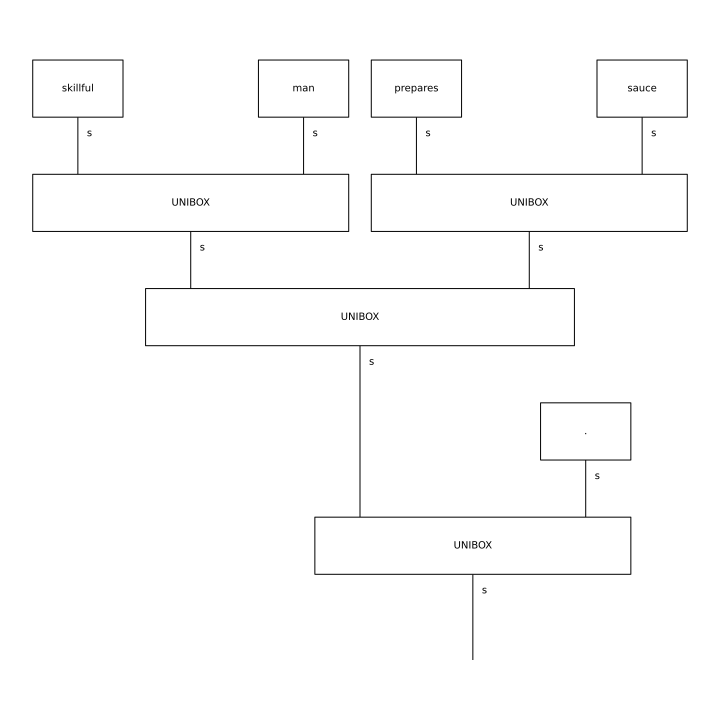
\includegraphics[width=\textwidth]{../test/output/treereader.pdf}
  \caption{ {\bf TreeReader example diagram}}
  \label{fig:treereader}
\end{figure} 
We use parsers to generate string diagrams, such as the {\it Bobcat} parser in the {\it lambeq} package which produced the string diagram in Figure \ref{fig:bobcat}. Alternatively, we can use trees for representing string diagrams.

\subsection{{\it TreeReader}}
The {\it TreeReader} class in the {\it lambeq} package is an alternative way of generating string diagrams using box representations. For example, the tree generated by the {\it TreeReader} in Figure \ref{fig:treereader} is not the same as the tree in Figure \ref{fig:bobcat} generated by {\it Bobcat} because {\it Bobcat} uses a more informed pregroup grammar for specific words. However, one could construct an equivalent tree using the TreeReader. While the documentation for generating trees using {\it TreeReader } to generate string diagrams was plentiful, I had a difficult time finding how to use a diagram generated by {\it TreeReader } for training a model.

\subsubsection{Problems with {\it TreeReader} and {\it stairs}}
Using the string diagrams generated by the {\it TreeReader} and {\it stairs} classes generate the following error:

\begin{verbatim}
  The arrow is ill-defined.
  Applying the functor to a box returns dom = Ty(),
  cod = s expected dom = s @ s, cod = s
\end{verbatim}
To debug this error, I first reverted to a previous version of {\it lambeq} and used the old backend for training the model. However, I ran into a similar implementation error. It's possible I missed a simple way of implementing {\it TreeReader}, but I digged through documentation for a while to no avail. The second thing I tried was to test implementations of the {\it stairs\_reader}, {\it spiders\_reader}, and {\it cups\_reader} classes. I found that the {\it cups\_reader}  works as expected despite using boxes, but the {\it stairs\_reader} breaks similarly to the {\it TreeReader}. Digging into when the dom changes, as indicated by the error, I found that the {\it then()} call in the \_\_rshift\_\_ operator is overwriting the dom but due to time constraints I decided to pursue the more familiar direction of generating custom string diagrams using cups. I will now demonstrate my contributions and present more hurdles to overcome for future work. 


\section{Methods}
In this section, I will describe all three readers I've implemented and the training process for the models.

\subsection{RandomTreeReader}
I first begin by implementing a random tree reader similar to the {\it TreeReader} in the {\it lambeq} package. The {\it RandomTreeReader} first tokenizes a sentence using the whitespace delimiter. Then, it builds the tree nodes by using a post-order traversal with a random midpoint in the list of tokens to separate the tokens into a left and a right subtree. I demonstrate the class in the following figure; both trees use the {\it RandomTreeReader} class on the same sentence and generate different trees.
\begin{figure}[t!]
    \centering
    \begin{subfigure}[t]{0.5\textwidth}
        \centering
        \includegraphics[width=\textwidth]{../test/output/random_1.pdf}
    \end{subfigure}%
    ~ 
    \begin{subfigure}[t]{0.5\textwidth}
        \centering
        \includegraphics[width=\textwidth]{../test/output/random_2.pdf}
    \end{subfigure}
    \label{fig:randomtrees}
    \caption{{\it RandomTreeReader} generates different trees for the same sentence ``mary prepares tasty dinner ."}
\end{figure}

\subsection{DeterministicTreeReader}
I implemented a {\it DeterministicTreeReader} to replace {\it TreeReader}. What makes it different is that the string diagrams generated are more akin to the string diagrams generated by {\it Bobcat} than {\it TreeReader} while still maintaining the tree structure of {\it TreeReader}. This implementation uses custom {\it TreeNode} classes for building a tree before the string diagram. After generating a list of words, the tree is constructed by passing in cup indeces to the {\it Diagram.create\_pregroup\_diagram} function.
The {\it DeterministicTreeReader} class is similar to the {\it RandomTreeReader} but instead of using a random midpoint, it uses the deterministic middle point for separating the tree.   The midpoint is the middle of the list of tokens. I demonstrate the class in Figure \ref{fig:deterministictrees}; both trees use the {\it DeterministicTreeReader} class on the same sentence and generate the same trees.

\subsubsection{Problems with {\it DeterministicTreeReader}}
The main problem with {\it DeterministicTreeReader} is that it doesn't use the {\it lambeq} backend for generating the trees. Due to time constraints, I could not familiarize myself with the backend to build a true extension of {\it lambeq}. However, I am confident that given more familiarity, I could add similar classes and improve {\it TreeReader} to work as expected. 

\subsection{{\it RandomTreeParser}}
Lastly, I implemented a {\it RandomTreeParser} as a random reader that generates random trees like  {\it RandomTreeReader} using string diagrams from words and cups similar to {\it DeterministicTreeReader} and {\it Bobcat}.  
\subsubsection{Problems with {\it RandomTreeParser}}
The main problem with {\it RandomTreeParser} is that the cups passed to {\it Diagram.create\_pregroup\_diagram} are reordered. Due to time constraints I could not fix this error. We can see in Figure \ref{fig:randomtreeparser} that the cups are randomly configured, though valid, but generate the same string diagram. 

\begin{figure}[t!]
    \centering
    \begin{subfigure}[t]{0.5\textwidth}
        \centering
        \includegraphics[width=\textwidth]{../test/output/randomParser_0.pdf}
        \caption{Cup indeces given as: [[0, 1], [3, 10], [4, 5], [7, 8], [6, 9], [11, 12], [2, 13], [15, 16]]}

    \end{subfigure}%
    ~ 
    \begin{subfigure}[t]{0.5\textwidth}
        \centering
        \includegraphics[width=\textwidth]{../test/output/randomParser_1.pdf}
        \caption{Cup indeces given as: [[0, 1], [3, 4], [2, 5], [7, 10], [8, 9], [11, 12], [6, 13], [15, 16]]}

    \end{subfigure}
    \caption{{\it RandomTreeParser} generates the same string diagrams for difference cup indeces on the sentence ``mary prepares tasty dinner ."}
    \label{fig:randomtreeparser}
\end{figure}

\subsection{Training the Models}
Despite the issues discussed with the readers, it is possible to train models using the readers. The training loss function is the Binary Cross Entropy loss function to train the model,
\begin{equation}
  \mathcal{L}(\yh, \y) = -\frac{1}{N}\sum_{i=1}^N \left[ \y_i \log(\yh_i) + (1-\y_i)\log(1-\yh_i) \right],
\end{equation}
which is minimized using the Adam optimizer. The model is trained on the MC dataset and validated on a validation subset. The model is trained for 50 epochs using a batch size of 30, learning rate of $3\times 10^-2$, and a random integer seed between $0$ and $100$.


\section{Results}

 The training results are provided for two models trained on both the {\it DeterministicTreeReader} and {\it RandomTreeParser} readers.

\begin{figure}[t!]
  \centering
\includegraphics[width=\textwidth]{../test/output/figure.pdf}
  \caption{Training results for the models trained on the {\it DeterministicTreeReader} and {\it RandomTreeParser} readers.}
  \label{fig:results}

\end{figure}

Figure \ref{fig:results} shows the training results for the models. The models trained on the {\it DeterministicTreeReader} and {\it RandomTreeParser} readers perform similarly. The models have very similar performance, likely due to the reodering of the string diagrams mentioned in the issues section for the {\it RandomTreeParser} reader. Both models quickly converge to 100\% accuracy within 20 epochs on the training sets. Both also achieve around 84\% accuracy on the final validation set.


\section{Discussion}
The original goal of this work was to demonstrate deterministic and random {\it TreeReader } classes for generating string diagrams for sentence classification. However, due to issues outlined in the background section, generate the string diagram using the {\it TreeReader} leads to errors during training. Therefore, three alternative readers are demonstrated, two of which are compatible with model training. Given more time, I would like to collaborate with the engineers who developed {\it lambeq} to learn how to faithfully implement {\it TreeReader} for training, properly define random cup index assignments. 

Overall, I spent approximately 20 hours on this project. I spent the most time on debugging my implementations of the string diagrams, learning about DisCoCat, and writing this report.

\section{Running the Code}
The code for this project is available in the {\it qnlp/} package directory. To run the code, first install the package in a virtual environment using the following commands: 
\begin{verbatim}
  python -m venv .env 
  source .env/bin/activate
  python -m pip install -e .
\end{verbatim}

Then, the following script can be run to train the models: 

\begin{verbatim}
  python test/testTorch.py
\end{verbatim}

To plot the training results:
\begin{verbatim}
  python test/testPlot.py
\end{verbatim}

To reproduce the errors mentioned in this work:
\begin{verbatim}
  python test/testErrors.py
\end{verbatim}

To generate/plot the string diagrams:
\begin{verbatim}
  python test/testReaders.py
\end{verbatim}



\end{document}
